\documentclass[zihao=false,fontset=windows]{ctexart}
% ctexart 不接受任意 pt 选项。正文改 {10pt}，方括号里是行距。
\usepackage{scrextend}
\changefontsizes[12pt]{10pt}

\usepackage[a4paper,left=2.35cm,right=2.35cm,top=1.7cm,bottom=1.9cm]{geometry}
\usepackage{xcolor}
\usepackage{graphicx}
\usepackage{amsmath,amssymb}
\usepackage{enumitem}
\usepackage{tabularx}
\usepackage{colortbl}
\usepackage{listings}
\usepackage{hyperref}
\usepackage[most]{tcolorbox}

\definecolor{feishuText}{RGB}{31,35,41}
\definecolor{feishuBlue}{RGB}{36,91,219}
\definecolor{feishuRed}{RGB}{216,57,49}
\definecolor{feishuGray}{RGB}{100,106,115}
\definecolor{feishuGray2}{RGB}{143,149,158}
\definecolor{feishuPinkBg}{RGB}{251,191,188}
\definecolor{quoteBar}{RGB}{51,112,255}
\definecolor{codebg}{RGB}{245,246,247}
\definecolor{codeborder}{RGB}{222,224,227}
\definecolor{inlinebg}{RGB}{242,243,245}
\definecolor{callRed}{RGB}{253,226,226}
\definecolor{callOrange}{RGB}{255,245,235}
\definecolor{callYellow}{RGB}{254,255,240}
\definecolor{callGreen}{RGB}{240,251,239}
\definecolor{callBlue}{RGB}{240,244,255}
\definecolor{callRedSoft}{RGB}{254,241,241}
\definecolor{callSun}{RGB}{255,255,204}
\definecolor{tableHead}{RGB}{242,243,245}
\definecolor{tableRule}{RGB}{222,224,227}
\definecolor{codeText}{RGB}{31,35,41}
\definecolor{codeKeyword}{RGB}{0,0,255}
\definecolor{codeComment}{RGB}{0,128,0}
\definecolor{codeString}{RGB}{163,21,21}

\setmainfont{Times New Roman}
\setCJKmainfont{Microsoft YaHei}[AutoFakeBold=2.2]
\setCJKsansfont{Microsoft YaHei}[AutoFakeBold=2.2]
\setCJKmonofont{Microsoft YaHei}[AutoFakeBold=2.2]
\setmonofont{Consolas}
\newfontfamily\emojifont{Segoe UI Emoji}

\hypersetup{
  colorlinks=true,
  urlcolor=feishuBlue,
  linkcolor=feishuBlue,
  unicode=true,
  pdftitle={Flamingo(2022, DeepMind)}
}

\setlength{\parindent}{0pt}
\setlength{\parskip}{0.42em}
\setlength{\fboxsep}{1.5pt}
\setlength{\emergencystretch}{3em}
\linespread{1.28}
\color{feishuText}
\arrayrulecolor{tableRule}
\urlstyle{same}

\setlist[enumerate]{label=\textcolor{feishuBlue}{\arabic*.}, leftmargin=1.7em, itemsep=0.22em, topsep=0.28em, parsep=0.08em, partopsep=0pt}
\setlist[itemize,1]{label=\textcolor{feishuBlue}{\textbullet}, leftmargin=1.35em, itemsep=0.18em, topsep=0.25em, parsep=0.06em, partopsep=0pt}
\setlist[itemize,2]{label=\textcolor{feishuBlue}{◦}, leftmargin=1.45em, itemsep=0.12em, topsep=0.15em}
\setlist[itemize,3]{label=\textcolor{feishuBlue}{\rule[0.18em]{0.38em}{0.38em}}, leftmargin=1.55em, itemsep=0.1em, topsep=0.12em}

\newcommand{\feiEmoji}[1]{{\emojifont #1}}
\newcommand{\incode}[1]{\colorbox{inlinebg}{\ttfamily\small #1}}
\newcommand{\bigmath}[1]{%
  \begin{center}\large$\displaystyle #1$\end{center}%
}
\newcommand{\codehead}{{\small\ttfamily\color{feishuGray}代码块}\par\vspace{-0.15em}}

\lstset{
  language=Python,
  basicstyle=\ttfamily\footnotesize\color{codeText},
  keywordstyle=\color{codeKeyword},
  commentstyle=\color{codeComment},
  stringstyle=\color{codeString},
  showstringspaces=false,
  breaklines=true,
  columns=fullflexible,
  keepspaces=true,
  tabsize=4,
  upquote=true,
  aboveskip=2pt,
  belowskip=0pt,
  xleftmargin=0pt,
  frame=none
}

\tcbset{
  feishubase/.style 2 args={
    enhanced,
    boxrule=0pt,
    arc=8pt,
    left=10pt,
    right=10pt,
    top=7pt,
    bottom=7pt,
    before skip=6pt,
    after skip=6pt,
    colback=#1,
    colframe=#1,
    before upper={\feiEmoji{#2}\hspace{0.45em}\ignorespaces}
  }
}
\newtcolorbox{feishubox}[2]{feishubase={#1}{#2}, breakable}
\newtcolorbox{feishuboxnb}[2]{feishubase={#1}{#2}}

\newtcolorbox{feishuquote}{
  enhanced,
  breakable,
  boxrule=0pt,
  leftrule=3pt,
  arc=0pt,
  colframe=quoteBar,
  colback=white,
  left=8pt,
  right=2pt,
  top=2pt,
  bottom=2pt,
  before skip=4pt,
  after skip=4pt,
  before upper=\color{feishuGray}
}

\newtcolorbox{feishucode}{
  enhanced,
  breakable,
  colback=codebg,
  colframe=codeborder,
  boxrule=0.6pt,
  arc=6pt,
  left=6pt,
  right=6pt,
  top=5pt,
  bottom=4pt,
  before skip=6pt,
  after skip=6pt
}

\begin{document}
{\zihao{1}\bfseries Flamingo(2022, DeepMind)\par}

\par\vspace{0.95em}\noindent{\zihao{3}\bfseries 模型结构}\par\vspace{0.28em}
\begin{center}
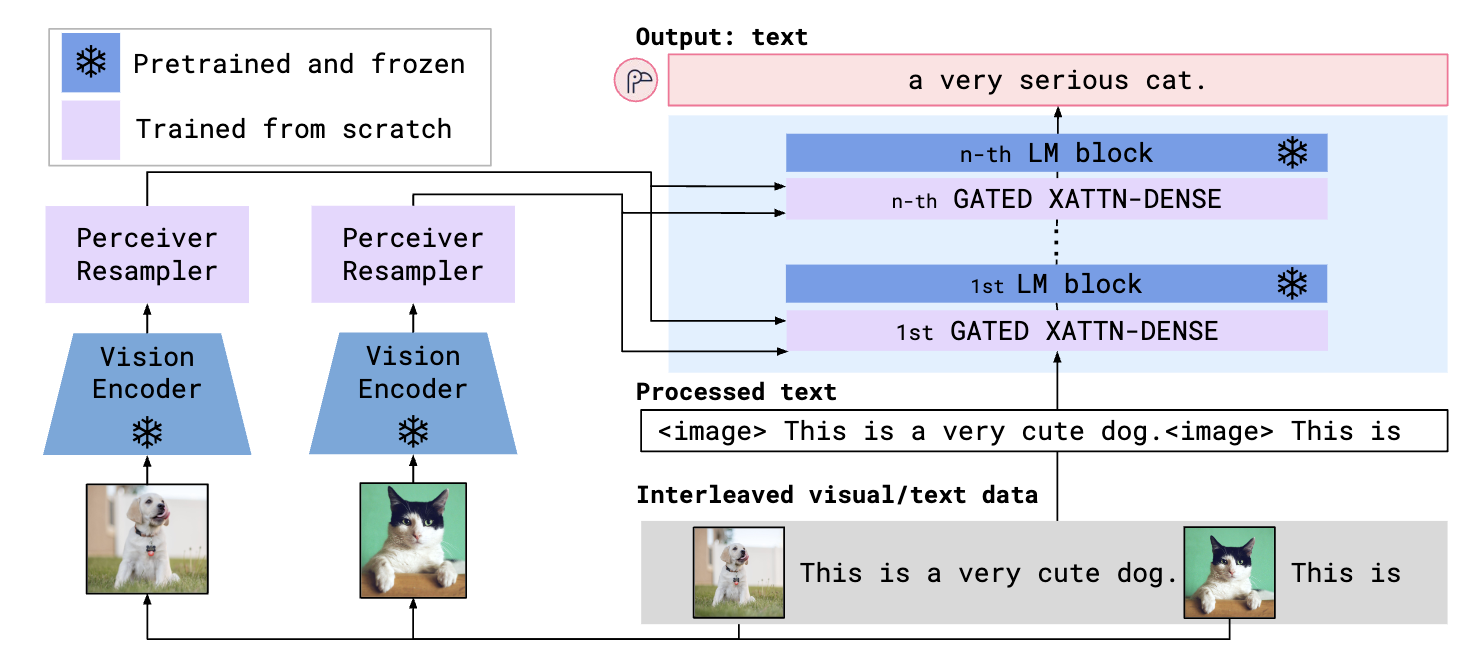
\includegraphics[width=0.98\textwidth]{images/2022-NeurIPS-Flamingo/fig-01.png}
\end{center}

\par\vspace{0.75em}\noindent{\zihao{4}\bfseries 输入输出格式}\par\vspace{0.28em}
输入text interleaved with images的形式，输出是text\par

\par\vspace{0.75em}\noindent{\zihao{4}\bfseries Vision Encoder}\par\vspace{0.28em}
视觉编码器采用NFNet（NormalizerFree ResNet），作者先在图文对数据上采用CLIP的方式对NFNet进行预训练。在Flamingo训练过程中，Vision Encoder权重固定·\par
如果视觉端输入是视频，则按照1 fps进行采样后将N帧进行视觉特征提取（若是图片输入，则N=1）。\par

\par\vspace{0.75em}\noindent{\zihao{4}\bfseries LLM}\par\vspace{0.28em}
1.4B, 7B, and 70B Chinchilla。并且这三个量级的LLM分别对应Flamingo-3B, Flamingo-9B, Flamingo-80B\par

\par\vspace{0.75em}\noindent{\zihao{4}\bfseries Perceiver Resampler}\par\vspace{0.28em}
Perceiver Resampler（感知重采样器） 可以接收任意多个的视频帧（如果是图像，可以视作是单帧视频），经过Vision Encoder提取特征，加上positional embedding 之后全部展平，得到一个视觉 token 序列 $X_f, X_f$ 的序列长度是任意的。还会有一个可学习的固定长度的 latent query 序列 $X$ 。 $X_f$ 和 $X$ 同时作为输入，送入到 Perceiver Resampler 中计算交叉注意力，注意力的 K 和 V 是 $X_f$ 和 $X$ 拼接而成，而 Q 就是 $X$ 。在经过多层 Attention＋FFW（其实就是FFN） 处理之后，输出固定长度（文中是 64）的 latent query，作为视觉表征。\par
\begin{center}
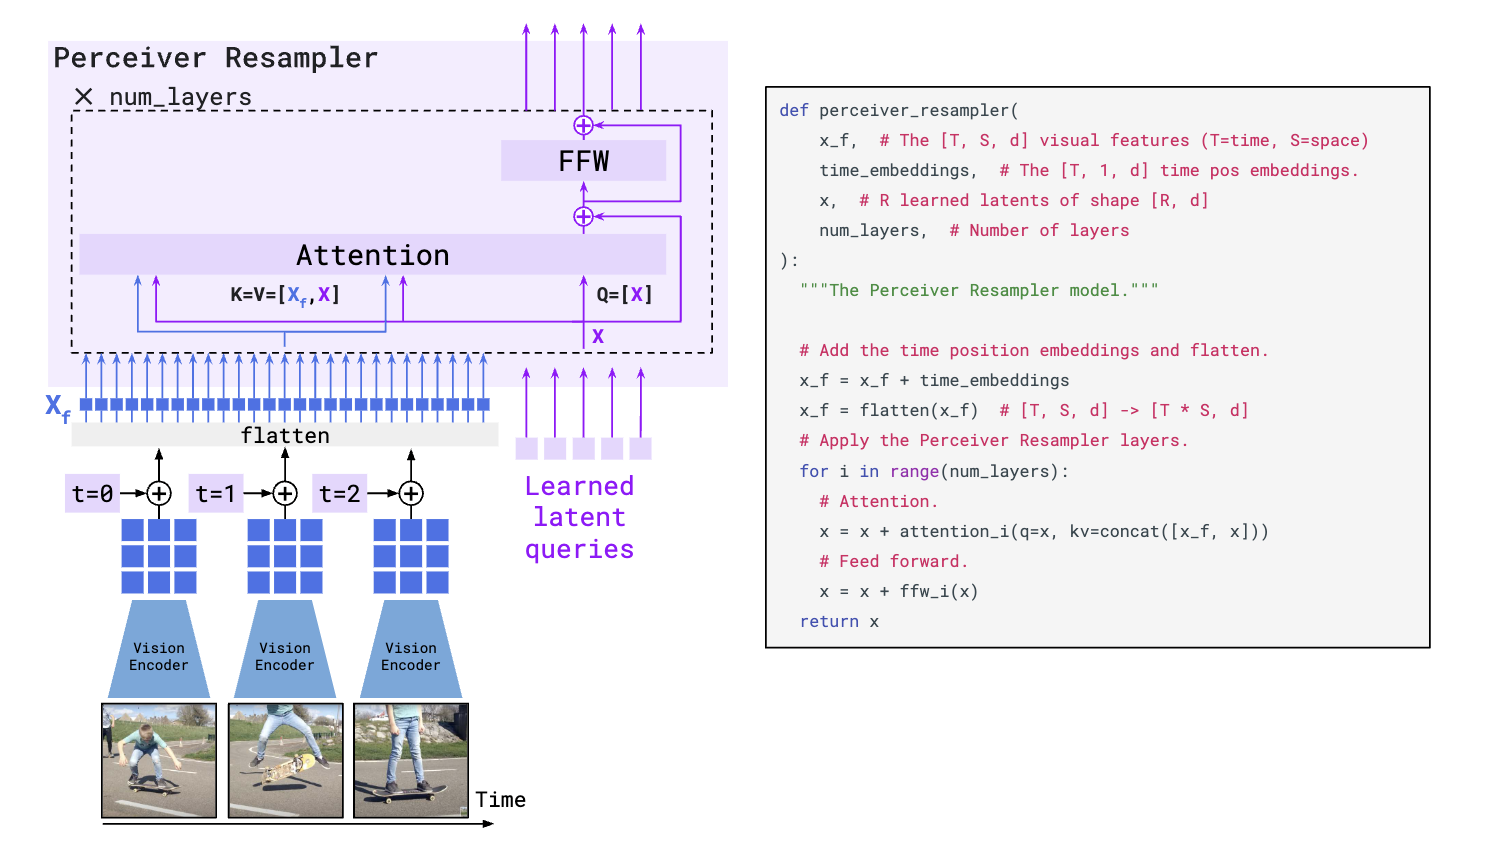
\includegraphics[width=0.98\textwidth]{images/2022-NeurIPS-Flamingo/fig-02.png}
\end{center}
注意这里的 positional embedding 只是 time embedding，即标识图片的时序信息，即图片来自哪一帧，这是因为单张图片内的空间位置信息在 vision encoder 中已经处理过了。\par
\begin{feishucode}
\codehead
\begin{lstlisting}
def perceiver_resampler(
        x_f, # The [T, S, d] visual features (T=time, S=space)
        time_embeddings, # The [T, 1, d] time pos embeddings.
        x, # R learned latents of shape [R, d]
        num_layers, # Number of layers
):
        """The Perceiver Resampler model."""
        # Add the time position embeddings and flatten.
        x_f = x_f + time_embeddings
        x_f = flatten(x_f) # [T, S, d] -> [T * S, d]
        # Apply the Perceiver Resampler layers.
        for i in range(num_layers):
                # Attention.
                x = x + attention_i(q=x, kv=concat([x_f, x]))
                # Feed forward.
                x = x + ffw_i(x)
        return x
\end{lstlisting}
\end{feishucode}

\par\vspace{0.75em}\noindent{\zihao{4}\bfseries Gated Xattn-Dense Layers}\par\vspace{0.28em}
Flamingo 将固定长度的视觉 query 注入到语言模型的方法称为 Gated xattn-dense，其详细结构示意图及伪代码如下图所示。具体来说，在预训练好的 LM 的各层交替地插入一些随机初始化的交叉注意力层。所谓 gated 门控，在每一新插入的层之后的残差链接之前的输出乘上一个可学习的 tanh gating，即 $\tanh (\alpha)=\frac{e^{\alpha}-e^{-\alpha}}{e^{\alpha}+e^{-\alpha}}$，其中 $\alpha$ 是一个可学习的标量值，初始值为 0 ，从而保证初始化时的输出与原 LM 一致。\par
\begin{center}
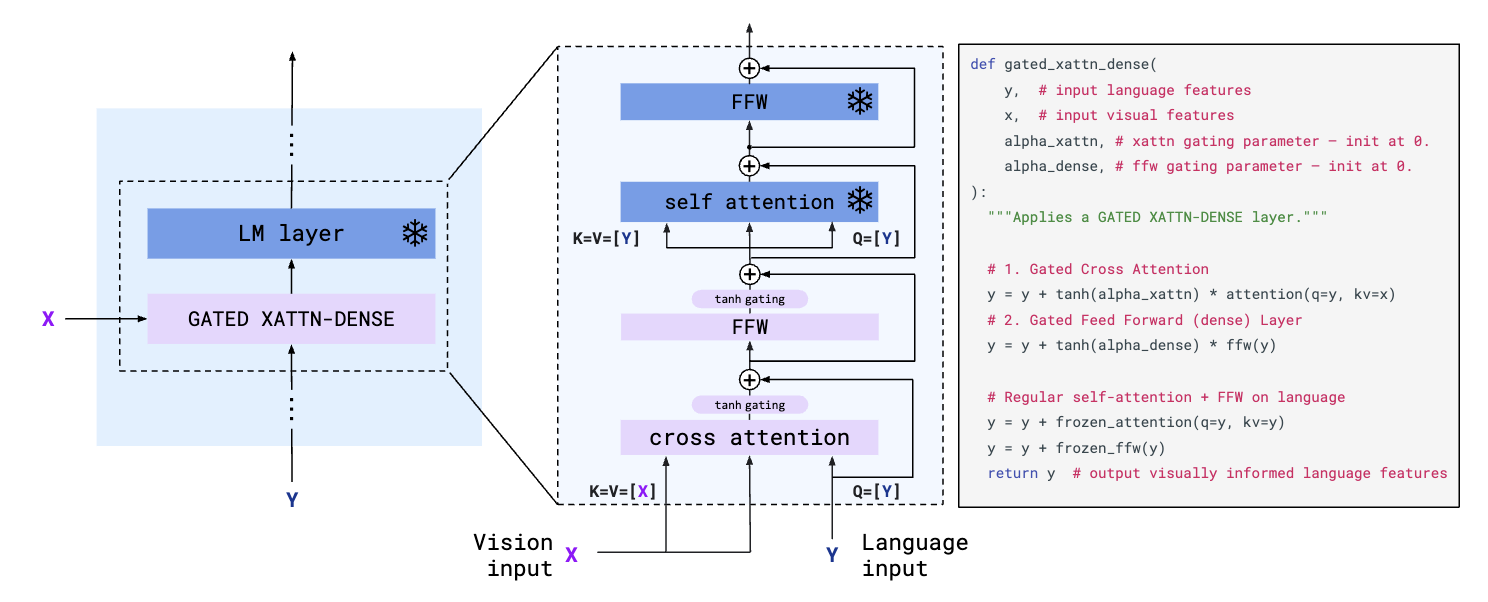
\includegraphics[width=0.98\textwidth]{images/2022-NeurIPS-Flamingo/fig-03.png}
\end{center}
\begin{feishucode}
\codehead
\begin{lstlisting}
def gated_xattn_dense(
        y, # input language features
        x, # input visual features
        alpha_xattn, # xattn gating parameter – init at 0.
        alpha_dense, # ffw gating parameter – init at 0.
):
        """Applies a GATED XATTN-DENSE layer."""
        # 1. Gated Cross Attention
        y = y + tanh(alpha_xattn) * attention(q=y, kv=x)
        # 2. Gated Feed Forward (dense) Layer
        y = y + tanh(alpha_dense) * ffw(y)
        # Regular self-attention + FFW on language
        y = y + frozen_attention(q=y, kv=y)
        y = y + frozen_ffw(y)
        return y # output visually informed language features
\end{lstlisting}
\end{feishucode}

\par\vspace{0.95em}\noindent{\zihao{3}\bfseries 训练}\par\vspace{0.28em}
Flamingo 的训练数据有三类：图文交错数据集、图像文本对数据集、视频文本对数据集。其中图文交错数据集是 Flamingo 数据的重点，其多模态 in-context learning（few-shot learning）的能力可以说主要就是来自图文交错数据。作者收集了一个大规模图文交错数据集 M3W ，通过解析 HTML 获取并标记图片在文本中的位置。\par
Flamingo 的训练还有一个关键点，就是如何处理图文交错数据。首先每张图片的特征用 vision encoder + resampler 处理得到固定长度的 token 序列，在文本序列中用 \incode{<image>} 这个 tag 来标记出图像的位置。值得一提的是，每个文本 token 只会 attend 到之前最近的一张图片，而不是所有之前的图片，之前的其他图片会被 mask 掉。\par
\begin{center}
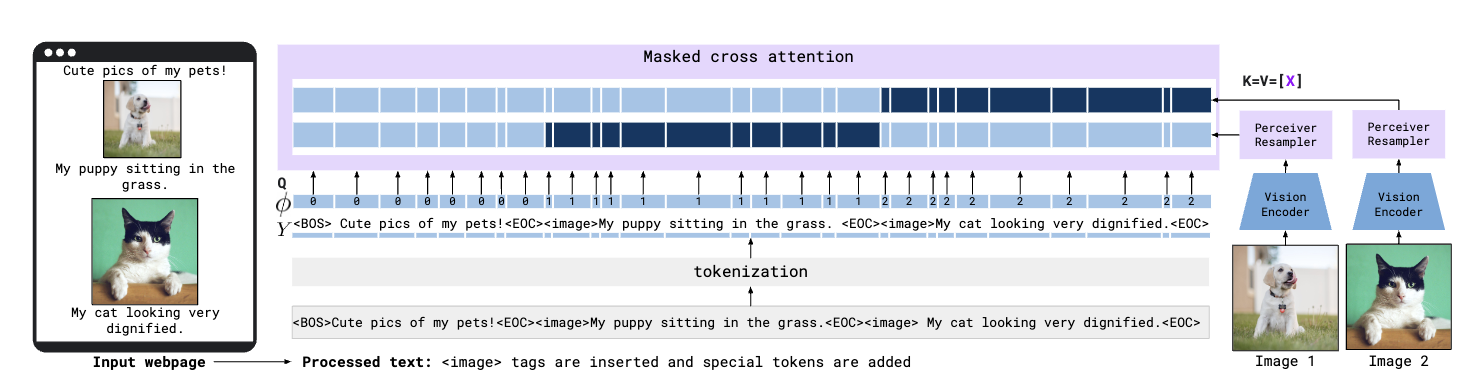
\includegraphics[width=0.98\textwidth]{images/2022-NeurIPS-Flamingo/fig-04.png}
\end{center}

\par\vspace{0.95em}\noindent{\zihao{3}\bfseries 实验}\par\vspace{0.28em}
模型在各个benchmark的表现：\par
\begin{center}
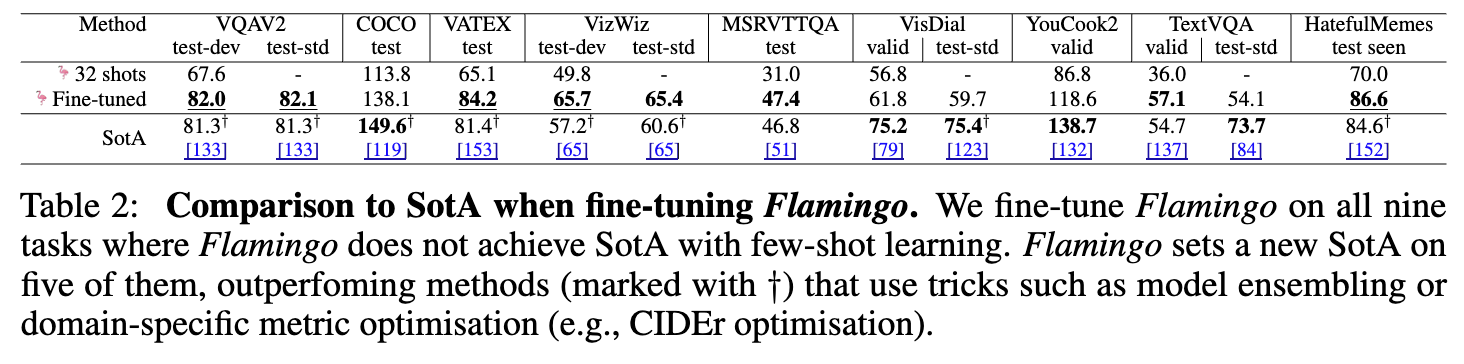
\includegraphics[width=0.98\textwidth]{images/2022-NeurIPS-Flamingo/fig-05.png}
\end{center}
Gated Xattn-Dense 可训练参数 $\alpha$随层深、训练step发生的变化。发现训练步数增加，层深增加，视觉语义融合加大。\par
\begin{center}
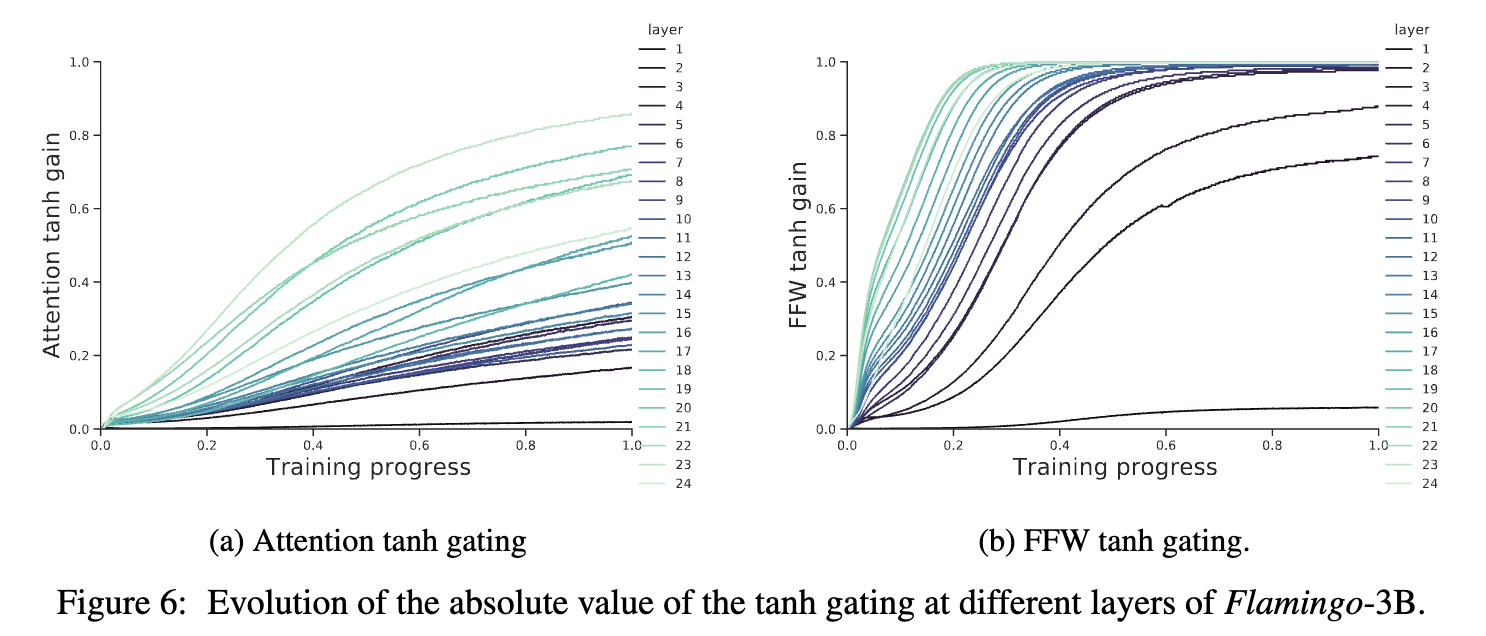
\includegraphics[width=0.98\textwidth]{images/2022-NeurIPS-Flamingo/fig-06.png}
\end{center}
再来看一下消融实验：\par
模型结构上来说，gating、resampler、cross attention layer 都是必须的\par
数据上来说 M3W 的缺失影响巨大\par
\begin{center}
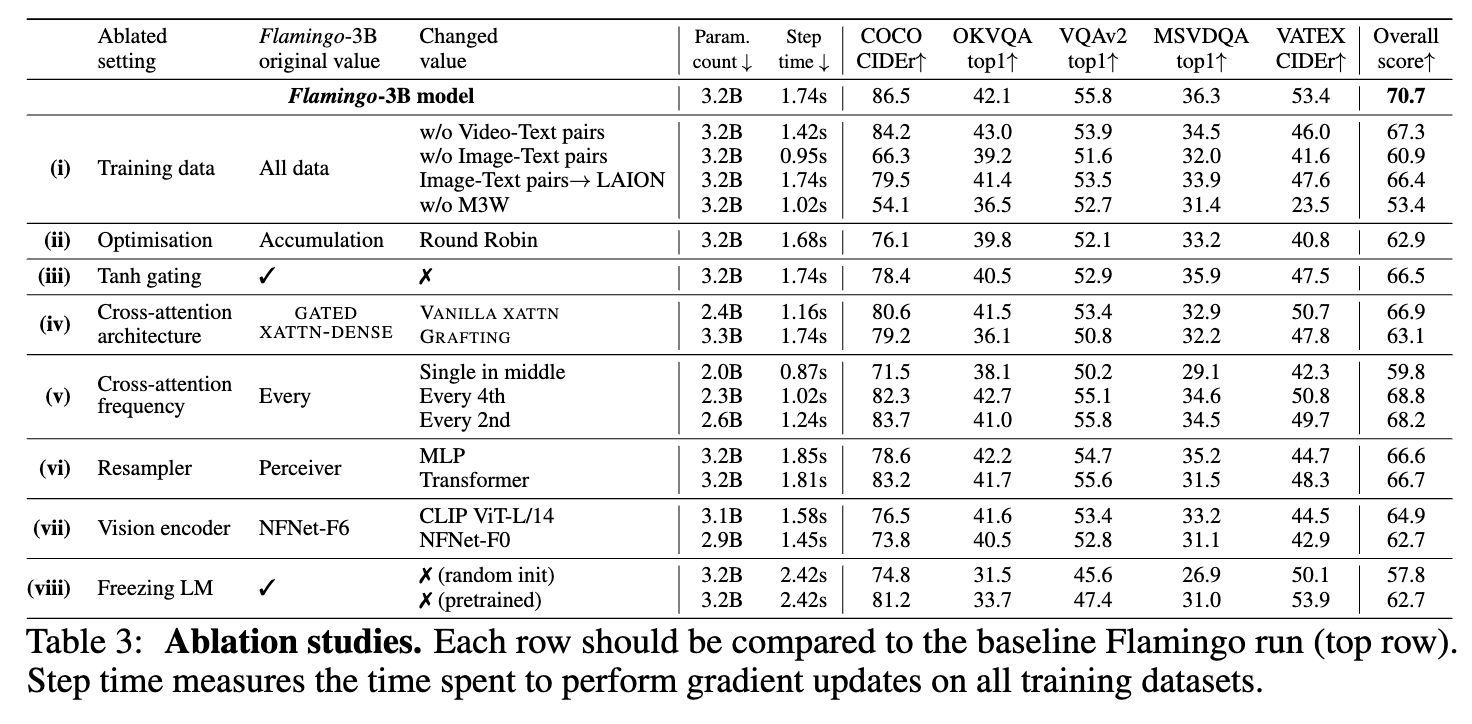
\includegraphics[width=0.98\textwidth]{images/2022-NeurIPS-Flamingo/fig-07.png}
\end{center}

\end{document}
